\subsection{Traffic Demand Per Subscriber}\label{subsec:behavior}

Internet usage throughout a day follows diurnal sleep-patterns, and researchers
have shown that such patterns are in fact correlated with GDP, Internet 
allocations, as well as electrical consumption of 
a region~\cite{ant-diurnal-web}. This makes the study of usage behavior 
extremely relevant to the governmental bodies responsible
for development, such as the FCC, when considering policy decisions.

To characterize diurnal user behavior as observed at the ISP, we first calculate
usage per subscriber (table ~\ref{tab:eval-criteria}), and then plot the median 
and 90\%-ile of total usage over a week for both \treatment{} and \control{}
sets (figure~\ref{fig:TS-data-rate-daily}).


We observe that the rise to the peak prime time hour usage on weekdays
is not plateaued like the pattern observed on weekends (and holidays).
A generic (median) weekday aggregate usage consists of a rise in usage that starts
early in the morning that builds up to the prime-time period, peaks, and then falls sharply.
We do not observe a trough in mid afternoon (between 2:00 PM -- 6:00 PM), as is usually
the case for overall usage observed at US Fixed access providers 
~\cite{sandvine20141h}.

\begin{figure}[ht]
\begin{minipage}{\linewidth}
  \centering
  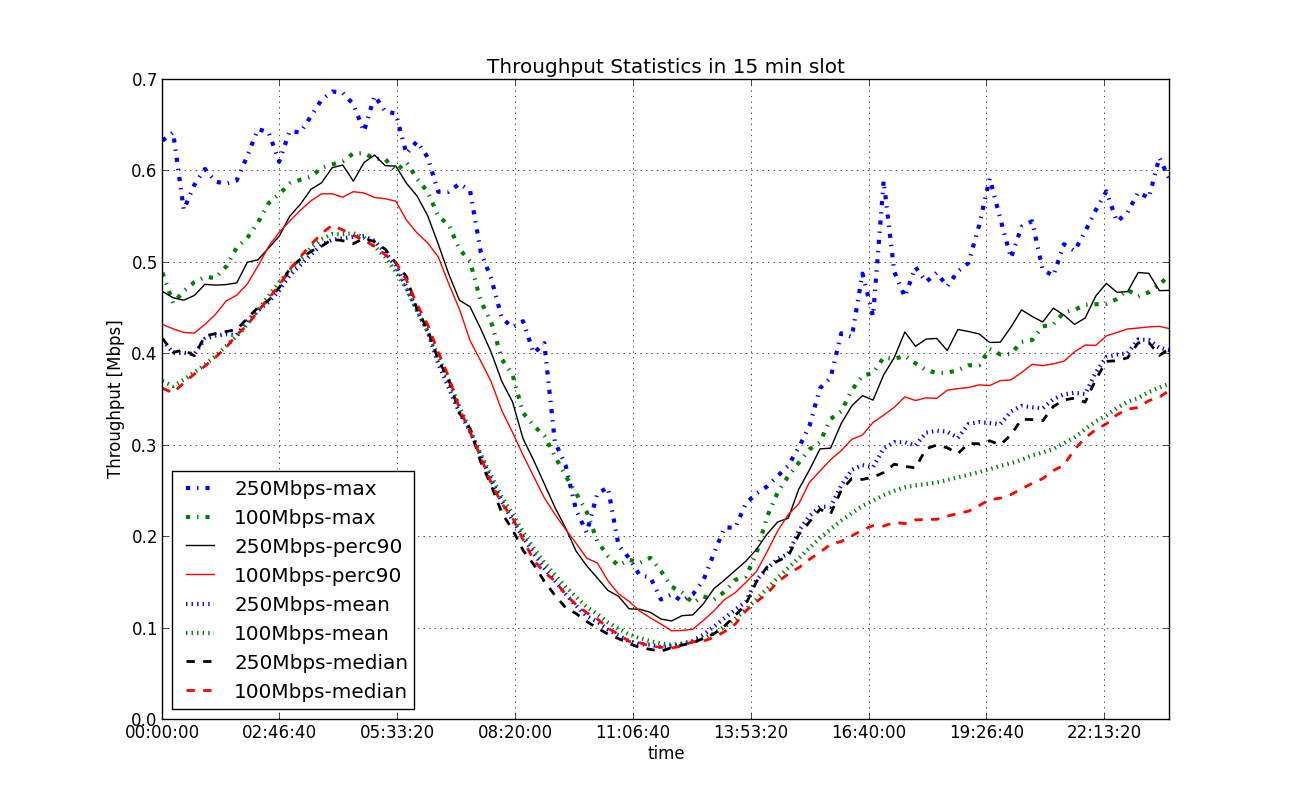
\includegraphics[width=\linewidth]{figures/describe-total-throughput-per-day[replace].png}
  \caption{agg (days) over means (devices): aggregate has no trough, peaks in the evening hours}
  %http://riverside.noise.gatech.edu:8083/separated/full/describe-total-throughput-per-day.png
  \label{fig:TS-data-rate-daily}
\end{minipage}
\end{figure}

Comparing the \test and \control sets, we observe that the median prime time and late night
behavior is very similar (7:00 PM -- 7:00 AM), but during off peak daytime (work) hours,
the \test set has a higher median than the \control set. There was no change in
prime time behavior in the evening, and an increased usage in off-peak daytime hours.

% EXPLAIN:
% LACK OF TROUGHS: users' behavior in higher tier bandwidth
% DISCREPANCY IN DAYTIME OFFPEAK: ???

figure~\ref{fig:CDF-data-rate-all} shows that
median utilization of household users is the same in both sets (50 kbps). A 
comparison
between the \test and \control set shows that there is no affect on the overall 
adoption.

\begin{figure}[ht]
\centering
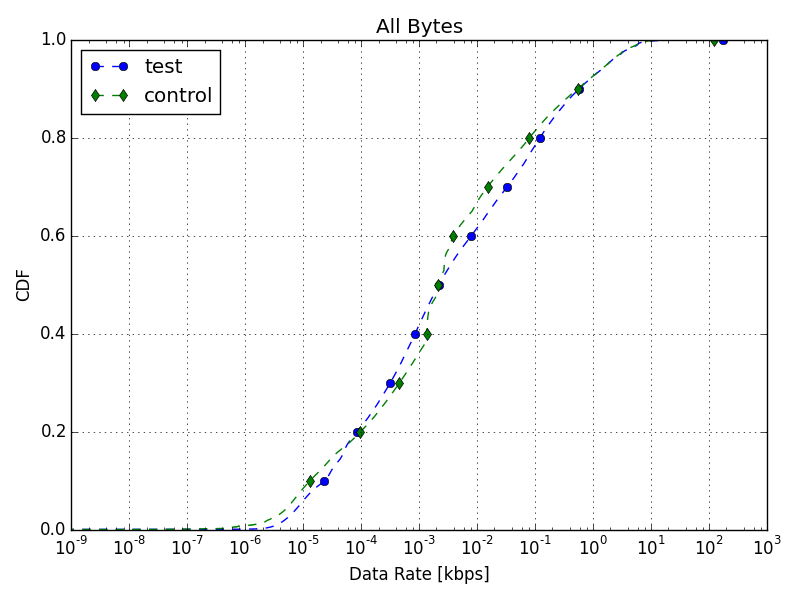
\includegraphics[width=0.90\linewidth]{figures/cdf-all-bytes.png}
  \caption{CDF of data rate per time slot for all devices (agg view of data): 
Overall not much change due to capacity increase. Median data rate ~ 2bps for 3 
months x thousands of devices!}
%http://sites.noise.gatech.edu/~sarthak/files/comcast/plots/full_dw/cdf-all-byte
% s.png
  \label{fig:CDF-data-rate-all}
\end{figure}

